\begin{problem}[1]
    $x^2 + 2xy + y^2 - x\sqrt{2} + y\sqrt{2} - 6 = 0$
\end{problem}

\begin{solution}[Solution]
    Strap in because this is going to be a long one. First thing I did here was use \textbf{theorem 3} to ascertain the end result of the graph of this guy. Really this isn't important to do this early on, but it can't hurt to know where we're going. \smallskip
    
    To do this let's first break down our coefficients. 
    
    \begin{align}
        A = 1 && B = 2 && C = 1 \\
        D = -\sqrt{2} && E = \sqrt{2} && F = -6
    \end{align}
    
    From here we use the equation from \textbf{theorem 3} and see what our relationship to 0 is! 
    
    \begin{align}
        B^2 - 4 \cdot A \cdot C &= 0 \\
        2^2 - 4 \cdot 1 \cdot 1 &= 0 \\
        4 - 4 &= 0
    \end{align}
    
    From this we know at the end of this insanity we will have a parabola! If we don't we can safely say we went wrong somewhere. Now, to officially get started. Next, we're going to make use of \textbf{theorem 2} to figure out our value of $\theta$. Why am I going backwards with theorems you may be wondering. It's because I have no idea what I'm doing. 
    
    \begin{align}
        cot(2\theta) &= \frac{A - C}{B} \\
        cot(2\theta) &= \frac{1-1}{2} \\
        cot(2\theta) &= 0 \\
        cot(\theta) &= 0 \; \text{when} \; \theta = \frac{\pi}{2} \\
        2\theta &= \frac{\pi}{2} \\
        \theta &= \frac{\pi}{4} + \frac{\pi}{2}k \; \text{for any integer k}
    \end{align}
    
    We choose $\frac{\pi}{4}$ here because it's easy and because I'm following the book and scared of what's to come. From here we can now tackle \textbf{theorem 1}. We have an angle to work with so we can actually define our x and our y. Or, at the least, start to.
    
    \begin{align}
        x &= x' \cdot \cos(\theta) - y' \sin(\theta) \\
        x &= x' \cdot \cos \left( \frac{\pi}{4} \right) - y' \sin\left( \frac{\pi}{4} \right) \\
        x &= \frac{x' \cdot \sqrt{2}}{2} - \frac{y' \cdot \sqrt{2}}{2}
    \end{align}
    
    \pagebreak
    
    \begin{align}
        y &= x' \cdot \sin(\theta) + y' \cos(\theta) \\
        y &= x' \cdot \sin \left( \frac{\pi}{4} \right) + y' \cos\left( \frac{\pi}{4} \right) \\
        y &= \frac{x' \cdot \sqrt{2}}{2} + \frac{y' \cdot \sqrt{2}}{2}
    \end{align}
    
    So, here's where things get fun. Before we proceed, for our own sanity we should go ahead and figure out in advance what $x^2$, $xy$, and $y^2$ are so we can plug those values instead of doing an absurd amount of work all at once. \bigskip
    
    Calculating $x^2$
    \begin{align}
        x^2 &= \left( \frac{x' \cdot \sqrt{2}}{2} - \frac{y' \cdot \sqrt{2}}{2} \right) \cdot \left( \frac{x' \cdot \sqrt{2}}{2} - \frac{y' \cdot \sqrt{2}}{2} \right) \\
        x^2 &= \frac{2 \cdot (x')^2}{4} - \frac{x'\sqrt{2} \cdot y'\sqrt{2}}{4} - \frac{x'\sqrt{2} \cdot y'\sqrt{2}}{4} + \frac{2 \cdot (y')^2}{4}
    \end{align}
    
    \[\boxed{x^2 = \frac{(x')^2}{2} - \frac{(2\cdot (x' \sqrt{2})) \cdot (2 \cdot (y' \sqrt{2}))}{4} + \frac{(y')^2}{2}}\]
    
    Calculating $y^2$
    \begin{align}
        y^2 &= \left( \frac{x' \cdot \sqrt{2}}{2} + \frac{y' \cdot \sqrt{2}}{2} \right) \cdot \left( \frac{x' \cdot \sqrt{2}}{2} + \frac{y' \cdot \sqrt{2}}{2} \right) \\
        y^2 &= \frac{2 \cdot (x')^2}{4} + \frac{x'\sqrt{2} \cdot y'\sqrt{2}}{4} + \frac{x'\sqrt{2} \cdot y'\sqrt{2}}{4} + \frac{2 \cdot (y')^2}{4}
    \end{align}
    
    \[\boxed{y^2 = \frac{(x')^2}{2} + \frac{(2\cdot (x' \sqrt{2})) \cdot (2 \cdot (y' \sqrt{2}))}{4} + \frac{(y')^2}{2}}\]
    
    Calculating $xy$
    \begin{align}
        xy &= \left( \frac{x' \cdot \sqrt{2}}{2} - \frac{y' \cdot \sqrt{2}}{2} \right) \cdot \left( \frac{x' \cdot \sqrt{2}}{2} + \frac{y' \cdot \sqrt{2}}{2} \right) \\
        xy &= \frac{2 \cdot (x')^2}{4} + \frac{x'\sqrt{2} \cdot y'\sqrt{2}}{4} - \frac{x'\sqrt{2} \cdot y'\sqrt{2}}{4} - \frac{2 \cdot (y')^2}{4}
    \end{align}
    \[\boxed{xy = \frac{(x')^2}{2} - \frac{(y')^2}{2}}\]
    
    That was a lot, but now this is where we really get going. What we need to do now is plug these values back into our original equation and see what it all boils down to. \pagebreak
    
    Substituting everything back into the original equation:
    
    \begin{align}
        0 &= x^2 + 2xy + y^2 - x\sqrt{2} + y\sqrt{2} - 6 \\
        0 &= \left( \frac{(x')^2}{2} - \frac{(2\cdot (x' \sqrt{2})) \cdot (2 \cdot (y' \sqrt{2}))}{4} + \frac{(y')^2}{2} \right) + \left( 2 \cdot \left( \frac{(x')^2}{2} - \frac{(y')^2}{2} \right) \right) + \\ 
        & \left( \frac{(x')^2}{2} + \frac{(2\cdot (x' \sqrt{2})) \cdot (2 \cdot (y' \sqrt{2}))}{4} + \frac{(y')^2}{2} \right) - \left( \left( \frac{x' \cdot \sqrt{2}}{2} - \frac{y' \cdot \sqrt{2}}{2} \right) \cdot \sqrt{2} \right) + \\
        & \left( \left( \frac{x' \cdot \sqrt{2}}{2} + \frac{y' \cdot \sqrt{2}}{2} \right) \cdot \sqrt{2} \right) - 6 
    \end{align}
    
    Okay, so that looks horrifying. I hate it. Thankfully it isn't quite as bad as it looks. I'll tell you this now, most of it will cancel. It's still quite an undertaking so how I'll do it is by simplifying it in pieces. I'll be taking bits that are similar in format, mushing them together and seeing what happens. Firstly we'll start with the two biggest chunks in the parentheses. I'll be referring to each chunk within parentheses as chunk 1, 2, 3, 4 and 5 for my own sanity. So the two big chunks will be chunks 1 and 3 respectively. 
    
    \begin{align}
        \text{Chunks 1 and 3} &= \frac{(x')^2}{2} - \frac{(2\cdot (x' \sqrt{2})) \cdot (2 \cdot (y' \sqrt{2}))}{4} + \frac{(y')^2}{2}  + \frac{(x')^2}{2} + \frac{(2\cdot (x' \sqrt{2})) \cdot (2 \cdot (y' \sqrt{2}))}{4} + \frac{(y')^2}{2} \\
        & \text{The big boys cancel out, leaving just the smaller fractions.} \\
        &= \frac{2(x')^2}{2} + \frac{2(y')^2}{2}
    \end{align}
    \[\boxed{\text{Chunks 1 and 3} = (x')^2 + (y')^2}\]
    
    See, that's not too bad. Chunk 2 simplifies very nicely as well! 
    
    \[\text{Chunk 2} = \left( 2 \cdot \left( \frac{(x')^2}{2} - \frac{(y')^2}{2} \right) \right)\]
    \[\boxed{\text{Chunk 2} = (x')^2 - (y')^2}\]
    
    Now it's just chunks 4 and 5.
    
    \begin{align}
        \text{Chunks 4 and 5} &= \left( \left( \frac{x' \cdot \sqrt{2}}{2} - \frac{y' \cdot \sqrt{2}}{2} \right) \cdot \sqrt{2} \right) + \left( \left( \frac{x' \cdot \sqrt{2}}{2} + \frac{y' \cdot \sqrt{2}}{2} \right) \cdot \sqrt{2} \right) \\
        &= \frac{x' \cdot 2}{2} - \frac{y' \cdot 2}{2} + \frac{x' \cdot 2}{2} + \frac{y' \cdot 2}{2} \\
        &= x' - y' + x' + y'
    \end{align}
    \[\boxed{\text{Chunks 4 and 5} = 2x'}\]
    
    Putting all the chunks together:
    \[(x')^2 + (y')^2 + (x')^2 - (y')^2 + 2x' - 6 = 0\]
    \[2(x')^2 + 2x' - 6 = 0\]
    
    \pagebreak
    
    Okay, this is now a quadratic! That means we're on the right track as this will give us a parabola. From here we just need to do some basic algebra. Thank goodness. Unfortunately we have a quadratic that can't be factored, so we will have to use the quadratic formula here. Our goal here is to, of course, figure out our x'-intercepts. These are different from x-intercepts as I will showcase later. 
    
    \begin{align}
        x' &= \frac{-6 \pm \sqrt{b^2 - 4 \cdot a \cdot c}}{2 \cdot a} \\
        &= \frac{-2 \pm \sqrt{2^2 - (4 \cdot 2 \cdot -6)}}{2 \cdot 2} \\
        &= \frac{-2 \pm \sqrt{52}}{4} \\
        &= \frac{-2 \pm 2\sqrt{13}}{4} \\
        x' &= \frac{-1 \pm \sqrt{13}}{2}
    \end{align}
    
    \medskip
    
    \centering $y' = 0$ when:
    \[\boxed{x' = \frac{-1 + \sqrt{13}}{2} \; \text{and} \frac{-1 - \sqrt{13}}{2} }\]
    \[\boxed{x' \approx 1.3 \; \text{and} \; -2.3 }\]
    
    We can quickly solve for our y'-intercept as well. We just set $x=0$
    
    \[2(0)^2 + 2(0) - 6 = y'\]
    \[y' = -6\]
    
    From here we just plot our answer. You'll notice my answer differs from the one in the book. The books parabola is negative whereas mine is positive. I'll be upfront here, I have absolutely zero idea where I went wrong and this problem is far too long for me to go back and find out. This was my result. \medskip
    
    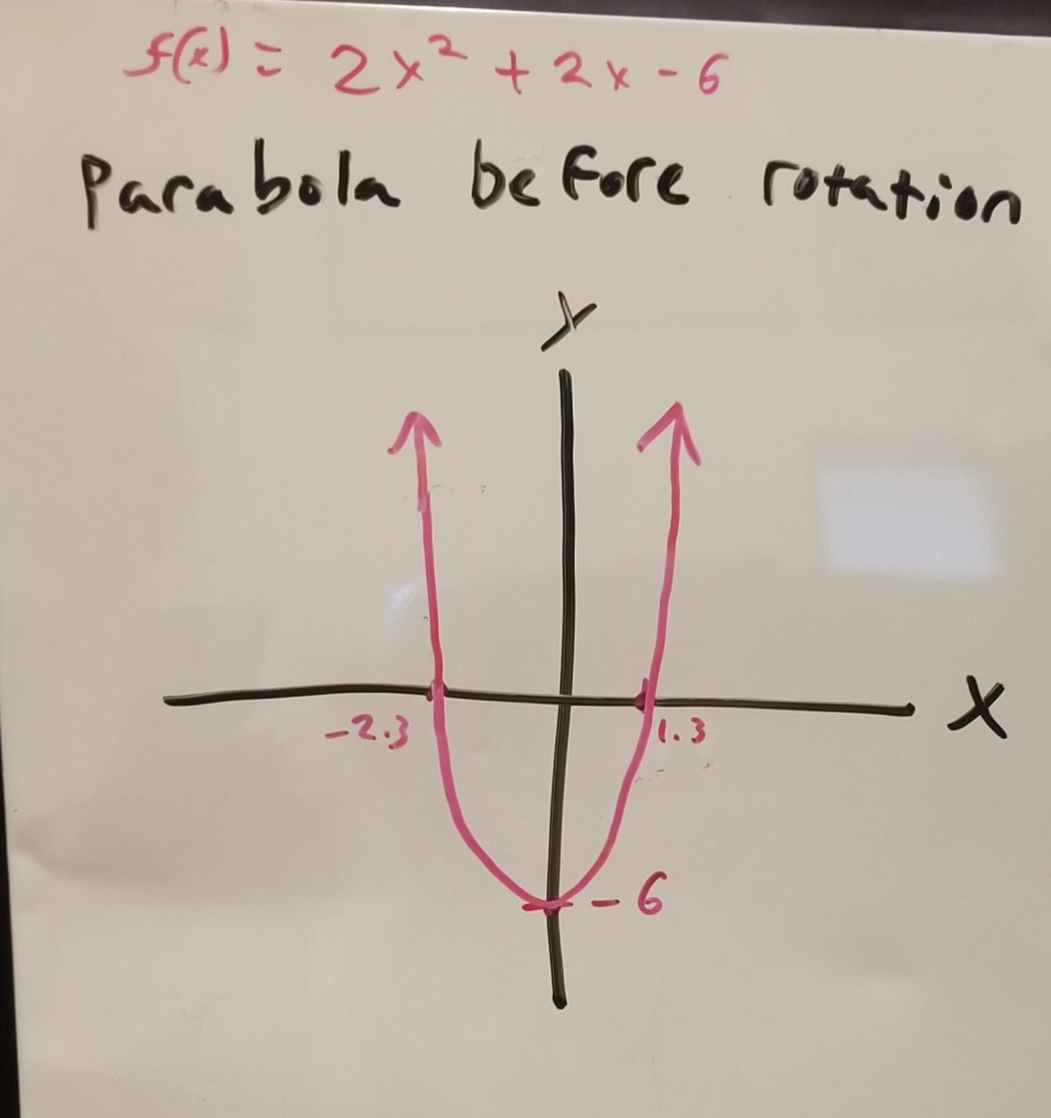
\includegraphics[scale=0.17]{images/pr1_prerotate.jpg}
    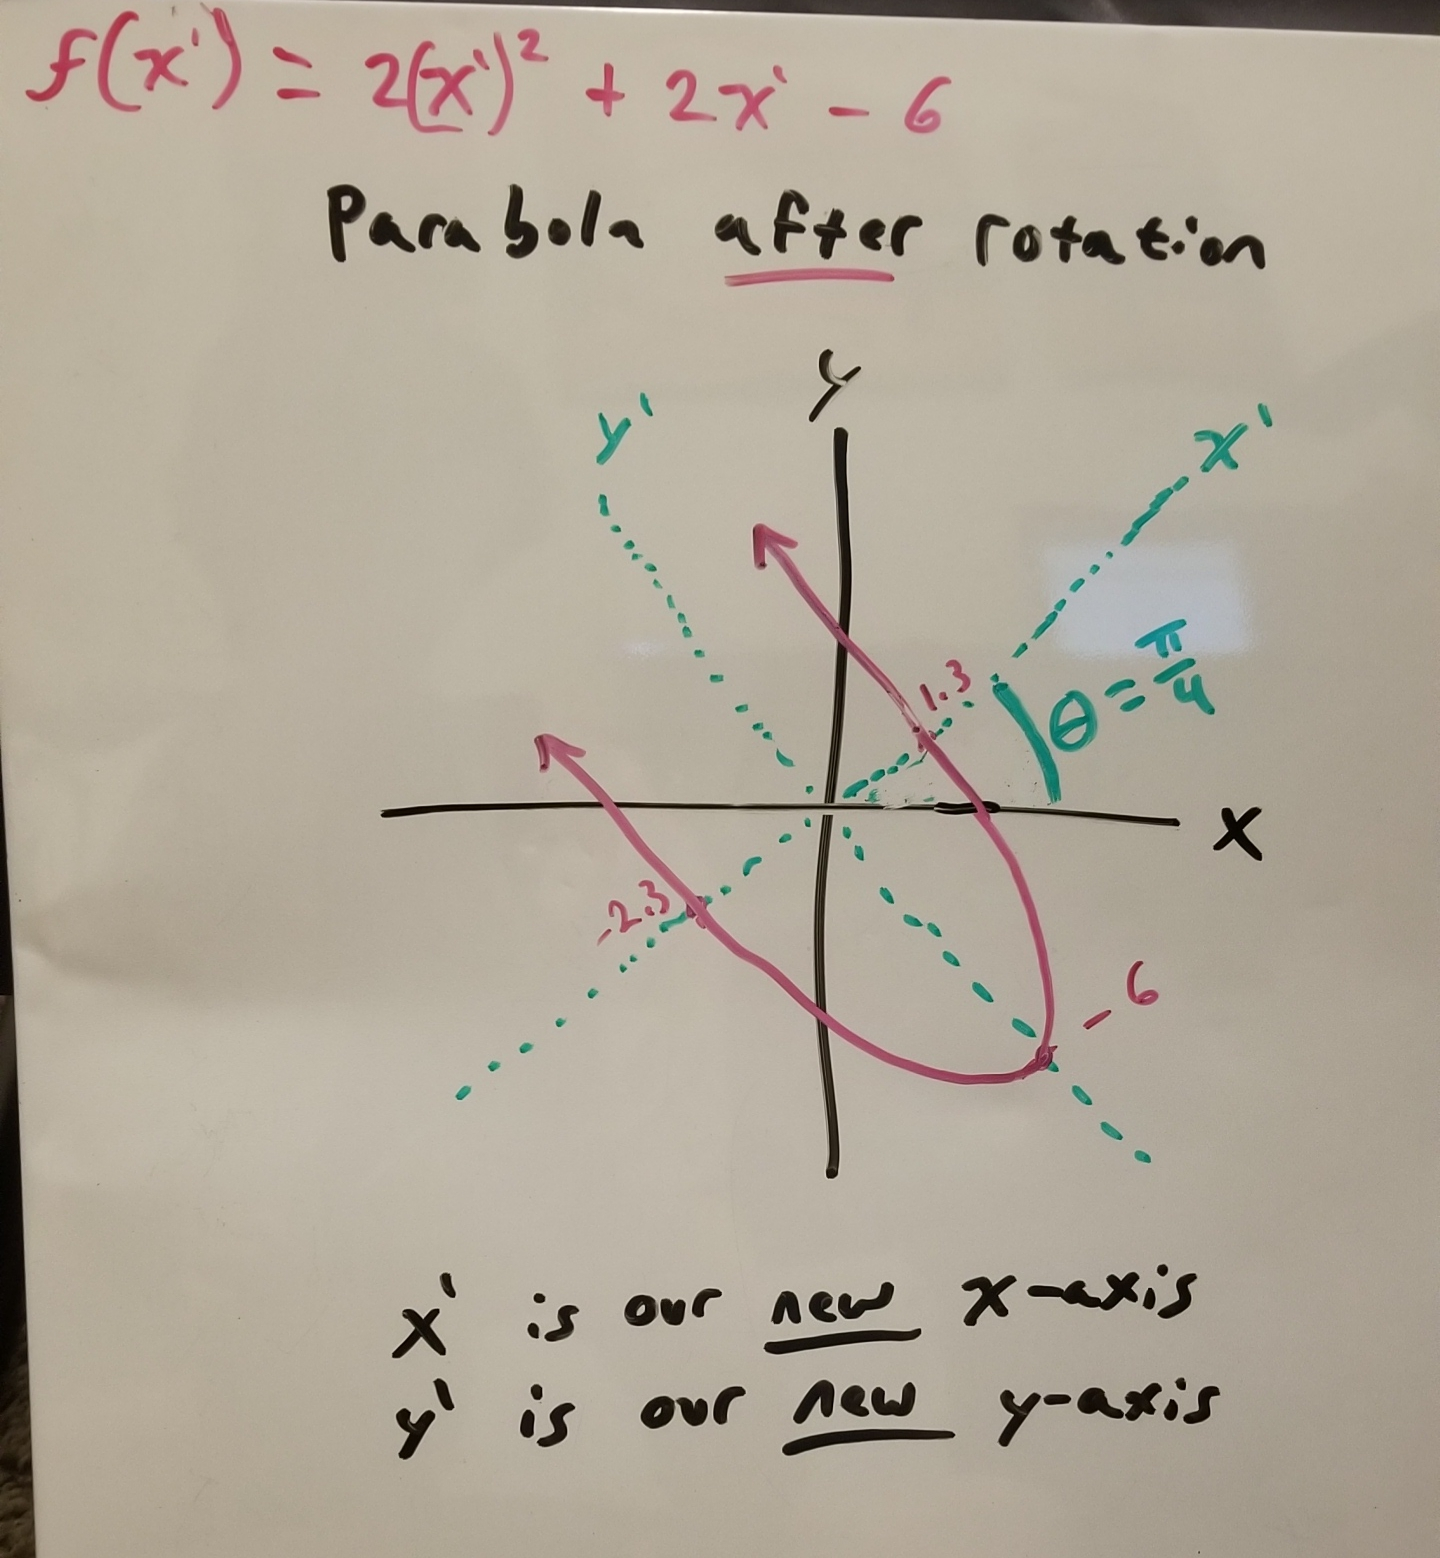
\includegraphics[scale=0.125]{images/pr1_postrotate.jpg}
\end{solution}